\documentclass{article}
\usepackage[margin=2cm]{geometry}
\usepackage{tabularx}
\usepackage{booktabs}
\usepackage{multirow}
\usepackage{enumitem}
\usepackage{url}
\usepackage{graphicx}
\usepackage{caption}
\usepackage{wrapfig}
\usepackage{setspace}
\usepackage{xcolor}
\usepackage{amsmath}
\usepackage{svg}
\usepackage{hyperref} % Required for hyperlinks
\usepackage{multicol} % this package is used to divide the document into multiple columns

\makeatletter
\renewcommand{\maketitle}{\bgroup\setlength{\parindent}{0pt}
\begin{center} % Center the title
  \Large\@title
  \newline
  \footnotesize\@author
\end{center}
\begin{flushright}
  \@date
\end{flushright}
\egroup}
\makeatother

% Adjust line spacing
\setstretch{0.9}

% Adjust paragraph spacing
\setlength{\parskip}{0pt}

\begin{document}

\title{Impact of Liquidity Pool Size on Trading Volume in BTC-ETH Pools}
\author{
  Team \#111 \\
   \scriptsize Matias Vizcaino (avizcaino3) | Walter Jack Simmons (wsimmons35) | Vítor de Matos Castilho (vcastilho3)
}
\date{20 July 2023}
\maketitle

\noindent
% {\setlength{\tabcolsep}{4pt} % Reduce column spacing


\begin{abstract}
  This paper investigates the dynamics of BTC-ETH liquidity pools on the Uniswap decentralized exchange, with a specific emphasis on the relationship between liquidity pool size and cumulative trading volume. Using an ordinary least squares regression model with lagged explanatory variables, we analyze the activity in the WBTC-WETH 3000 and 500 tick pools on Uniswap v3. We employ a data-driven approach, engineering features from Uniswap and Etherscan data, and take into account spillover effects from the Binance centralized exchange. Our findings confirm a direct correlation between liquidity pool size, increased mint frequency, immediate trading volumes, and cumulative trading volume. We also identify a significant spillover effect from centralized exchange activity on decentralized exchange pools. These insights offer important strategic guidance for liquidity providers, traders, and architects of decentralized exchanges. However, the potential multicollinearity of features and a predominantly linear modeling assumption call for caution in interpretation. Future work should consider employing nonlinear models and exploring other factors such as price divergences, impermanent loss, and inherent risk factors.
\end{abstract}
  
\section*{\textbf{Introduction}}

Decentralized Finance (DeFi) has rapidly evolved into a crucial segment of the blockchain ecosystem, contributing significantly to the democratization of financial services. At its core, DeFi is governed by a network of decentralized exchanges (DEXs), such as Uniswap, which rely extensively on liquidity pools for the efficient operation of trading activities. Liquidity pools, empowered by an automated market maker model, are one of the vital cogs in the DeFi machine, underpinning the entire transaction mechanism on these platforms\cite{Miori2022,Aigner2021,Xu2023}.

Given the centrality of liquidity pools in the DeFi landscape, understanding their dynamics and operational parameters is crucial. Notably, the WBTC-WETH liquidity pools on Uniswap serve as a significant focus, due to the considerable trading volume and liquidity they command. Therefore, this study delves into the exploration of these liquidity pools, investigating their intrinsic dynamics and external influences.

This study investigates these pools, specifically how pool size affects trading volume. Our research and code offers insights and practical value for liquidity providers, traders, and DeFi platform architects. Further research could benefit from broader analysis, exploration of additional variables, and consideration of non-linear models and industry events.

\section{\textbf{Uniswap Liquidity Pools: An Overview}}

Various DeFi platforms, including Uniswap, cater to unique needs within the blockchain ecosystem\cite{Xu2023}. Uniswap, a widely-used Ethereum-based DEX, employs a Constant Product Market Maker (CPMM) model supporting a broad spectrum of Ethereum-native and wrapped non-native asset trades\cite{Miori2023, Heimbach2022}.

Uniswap v3 further refined this model with "virtual" and "real" reserves, enabling more efficient capital usage and offering liquidity providers customization options for their price exposure\cite{Elsts2021}. The CPMM equation is pivotal to this:

\[x \cdot y = k \quad \text{and} \quad price = \frac{y}{x}\]

where \(x\) and \(y\) represent token quantities in the pool and \(k\) maintains the constant product\cite{Makarov2022,Miori2023}.

Operating without a central authority, Uniswap offers privacy, fund control, and a variety of tokens\cite{Miori2023}. In Uniswap transactions, "swaps" involve trading one token for another, while "mints" and "burns" pertain to liquidity providers adding or withdrawing funds from a pool respectively. Mints create liquidity tokens representing a provider's pool share, and burns destroy these tokens to facilitate fund withdrawal. Despite its advantages, DEXs pose impermanent loss risks to liquidity providers, a contrast to centralized exchanges which, while offering higher transaction speeds, can present security issues\cite{Aigner2021, Heimbach2022, Makarov2022}.

WBTC-WETH represents a liquidity pool between Wrapped Bitcoin (WBTC) and Wrapped Ethereum (WETH) on the Uniswap platform. WBTC is an ERC-20 token on the Ethereum blockchain that represents Bitcoin (1 WBTC equals 1 BTC). Similarly, WETH is an Ethereum token that represents Ether. These "wrapped" versions allow Bitcoin and Ether to be traded more quickly on the Ethereum blockchain and enable holders to interact with smart contracts and decentralized applications (dApps).

Uniswap v3 allows liquidity providers to set custom price ranges for their capital, indicated by ticks. These ticks influence capital efficiency and require active management\cite{Elsts2021}. The study focuses on WBTC-WETH 3000 and 500 pools, which differ in their tick spacing, impacting capital efficiency, potential returns, and slippage for liquidity providers and traders.

\section{\textbf{Analytical Methodology}}

A thorough analysis of the interconnectedness between Uniswap v3 WBTC-WETH exchange and a systematic selection for a subsets of pools of 3000 and 500 ticks for analysis is required. This will be done over different time periods, using similar methodologies as found in recent studies \cite{Miori2022}. The relationship between liquidity, trading volume, and price stability in pools will be examined, along with an investigation of how liquidity pool size impacts trading volume.

\begin{table}[htbp]
  \centering
  \small
  \begin{tabularx}{\linewidth}{|>{\raggedright\arraybackslash}X|}
  \hline
  \textbf{Feature Engineering:} Our models' predictive power was enhanced by creating new features from existing data\cite{Miori2023}. This process effectively captured crucial information about liquidity pool dynamics, spillover effects, and price divergences. \\
  \hline
  \textbf{Modelling and Optimization:} Through the application of Ordinary Least Squares (OLS) regression, we examined the relationship between liquidity pool size and trading volume, which offered profound insights into their interplay\cite{Miori2023}. Model performance was assessed using metrics such as R-squared, while we optimized feature selection, corrected multicollinearity, and explored alternative functional forms for improved model accuracy and interpretability\cite{Miori2023}. \\
  \hline
  \textbf{Innovations:} Building on the reference paper, we implemented the underlying code in Python, thus creating a robust data model to explore interactions between two liquidity pools more effectively\cite{Miori2023}. Furthermore, we developed a mathematical language to facilitate the data engineering aspects of the data model\cite{Miori2023}. \\
  \hline
  \end{tabularx}
  \caption{Analytical Techniques and Main Contributions}
  \label{fig:analytical-techniques}
  \end{table}
  
  Substantial accomplishments were achieved at each of our research stages, leading to a robust analysis framework and valuable initial results\cite{Miori2023}.

  \begin{table}[htbp]
  \centering
  \small
  \begin{tabularx}{\linewidth}{|>{\raggedright\arraybackslash}X|}
  \hline
  \textbf{Data Collection:} We sourced data from multiple APIs (Uniswap, Binance) successfully, and associated this data with Ethereum block numbers for consistent time measurement. \\
  \hline
  \textbf{Data Preprocessing:} We maintained data consistency, addressed discrepancies from different sources, and efficiently cleaned, formatted, and handled missing values in the dataset. \\
  \hline
  \textbf{Exploratory Data Analysis (EDA):} Utilizing EDA, we generated descriptive statistics, visualizations, and correlation analyses. This approach facilitated the identification of trends, outliers, and the relationships between variables. \\
  \hline
  \textbf{Final Analysis and Conclusions:} We articulated our findings and conclusions, providing quantitatively-driven insights with the potential to enhance liquidity provision, optimize trading strategies, and improve the efficiency of DeFi marketplaces. \\
  \hline
  \textbf{Confirmation of Results:} Our results largely coincide with those in the reference paper, with minor discrepancies likely due to the techniques used and features available. Notably, we utilized fewer features and feature categories than the reference paper, which might explain the minor divergences observed in our results\cite{Miori2023}. \\
  \hline
  \end{tabularx}
  \caption{Supporting Work and Confirmation of Results}
  \label{fig:approach-accomplishments}
  \end{table}

Our work provides a significant contribution by offering an open framework that allows other researchers and professionals to conduct further research in this field. This outcome not only answers our problem statement but also opens avenues for future exploration\cite{Miori2022}.

\subsection{\textbf{Challenges and Insights}}

Our main challenges were data collection and processing due to intricate engineering and the rate limits of the Etherscan free-tier API\cite{etherscanAPI}. Nonetheless, we overcame these hurdles and made significant progress in understanding liquidity pool dynamics\cite{Miori2022,Aigner2021,Miori2023}.

We embraced two time concepts—"trading clock" and "time horizon"—which enabled us to thoroughly explore both short and long-term trends. This detailed analysis offered invaluable insights for decision-making and risk management in the DeFi ecosystem\cite{Miori2022}.

We successfully addressed complexities in understanding entry-level liquidity pool mathematics and integrated the associated formulas into calculations.py functions. This step significantly enriched our feature derivation and bolstered our overall analysis\cite{Elsts2021,Aigner2021}.
For instance, we tackled the complexity of tick math, which involves mapping discrete ticks to continuous prices. This step, guided by the Uniswap v3 liquidity math paper, was essential for interpreting Uniswap data and indeces \cite{Elsts2021}. In addition, we adjusted raw price ratios for token decimals to get human-readable prices, a process critical for presenting our analysis \cite{Elsts2021}.

\textbf{Key Note:} Our models and code implementation have been designed with a focus on programming and data structure, and while they provide valuable insights, further improvement is needed to enhance the accuracy and completeness of our results. Due to the novelty of the topic and methodologies, we encourage peer review and rigorous testing of our calculations.py module, as well as a deeper understanding of the underlying liquidity mathematics as outlined in the Uniswap v3 liquidity math paper \cite{Elsts2021,Miori2023}.

\section{\textbf{Engineering Ecosystem}}

Data engineering and feature extraction are crucial elements for building robust predictive models. In the case of analyzing BTC-ETH trading volume on Uniswap, several aspects of data must be considered.

First, let's consider the nature of the data we are dealing with. Uniswap is a decentralized exchange that operates on an automated market-making (AMM) model, and its Version 3 (v3) utilizes a novel mechanism of concentrated liquidity pools. The structure and dynamics of these liquidity pools play a crucial role in trading volumes \cite{Miori2023}. We must extract relevant data from these pools, including their sizes, trading volumes, and related metrics, for accurate analysis. Understanding DeFi's goals and mechanisms from a broad perspective is also valuable \cite{Makarov2022}.

Moreover, it's important to incorporate data from different sources, considering not just the pools of interest but also neighboring pools and other prominent exchanges such as Binance. This kind of broad-spectrum data helps in capturing spillover effects, which are significant drivers of trading volume \cite{Miori2023}. For example, we could study the effects of trading volume and the activities from interconnected DeFi protocols and stablecoins \cite{Miori2022}.

Feature selection is a crucial part of the process. Stepwise regression can be an effective tool for optimizing the model and refining the set of independent variables \cite{Miori2023}. We should also account for factors like network effects, economies of scale, and concentration issues that can influence liquidity provision \cite{Makarov2022, Miori2022}.

From a risk perspective, we should ideally account for external risks to liquidity providers like arbitrage opportunities, fraudulent DEXs, regulatory risks, censorship risks, etc. \cite{Aigner2021}. Systemic risks from interconnected DeFi protocols and stablecoins could also impact trading activity \cite{Makarov2022}. Additionally, economic risks like yield dilution, conversion risk, exchange risk, counterparty risk, and liquidation risk pose challenges and should be considered \cite{Xu2023}.

For the implementation part, we can take advantage of mathematical equations and formulations. For example, we could use equations to calculate the amounts of assets based on liquidity, price range, and the current price \cite{Elsts2021}. Formulas for calculating impermanent loss and changes in holdings after a price change could also be useful in the analysis of this problem \cite{Elsts2021, Aigner2021, Heimbach2022}.

\subsection{\textbf{Data Sources}}

In line with the \textit{"DeFi modeling and forecasting trading volume" (2023)} study\cite{Miori2023}, we gathered and structured trade data spanning a minimum of 6 months. Further details on information gathering and engineering involved can be found in our GitHub repository\cite{TeamRepo}. 

Our analysis incorporates information from the below sources.

We limit the CEX data to consider only WBTC-WETH 3000 pool and 500 pool activity.

\begin{table}[ht]
  \centering
  \small
  \begin{tabular}{|p{0.15\linewidth}|p{0.30\linewidth}|p{0.5\linewidth}|}
  \hline
  \textbf{Source} & \textbf{Description} & \textbf{Data} \\
  \hline
  Uniswap's The Graph API\cite{uniswapAPI} & This API offers transaction details, trading volumes, and block data from Uniswap v3 liquidity pools. & Includes transaction IDs, timestamps, amounts, USD equivalents, and other related data. \\
  \hline
  Etherscan API\cite{etherscanAPI} & Utilized to extract corresponding transaction data from Etherscan based on transaction hashes. & Block hashes, block numbers, sender addresses, gas details, transaction hashes, and other relevant information. \\
  \hline
  Binance\cite{binanceData} & Provides Centralized Exchange (CEX) data for ETHBTC trades. Data was obtained via scripts from Binance's GitHub repository. & Contains detailed data about each trade performed on the Binance platform, including trade prices, quantities, timestamps, and buyer/seller characteristics. \\
  \hline
  \end{tabular}
  \caption{Dataset Source Description}
  \label{tab:dataset-description}
  \end{table}

\subsection{\textbf{Key Variables}}

\textbf{Target Variable:} The key dependent variable in our study is the trading volume of liquidity pools (amountUSD) over specific blocks. We propose several models for different time horizons to investigate how the relationships evolve over time.

\textbf{Independent Variables:} Constructed from various features and are grouped as follows:

\begin{enumerate}[label=\arabic*. ,itemsep=0pt, topsep=0pt]
\item \textbf{Direct Pool Features (41):} Measures such as volatility, rate, number of trades, and average trade size.
\item \textbf{CEX Spillover Effects (6):} Variables like actual coin trade volume on Centralized Exchanges (CEX), which can influence liquidity pools on decentralized platforms.
\end{enumerate}


\section{\textbf{In-Depth: Feature Engineering}}

Feature engineering is key in deciphering the intricate dynamics between variables in our analysis, with particular focus on temporal patterns in the DEX pools and the influence of CEX activities. We define the sequence of blocks within our scope as $B$ and the total number of these blocks as $K$. For the construction of a time-series model, "Reference Blocks" act as time markers, identified by Mint Operations in Uniswap DEX. They are classified into "same" and "other" pools and arranged in reverse chronological order.

\begin{equation}
B = \{b_k\}_{k=1}^{K} \text{ with } b_k \text{ a block within the scope of analysis}
\end{equation}

\begin{equation}
R_{s} = \{b_{s}\}_{s=1}^{S} \text{ with } b_{s} \text{ a reference block in the "same" pool}
\end{equation}

\begin{equation}
R_{o} = \{b_{o}\}_{o=1}^{O} \text{ with } b_{o} \text{ a reference block in the "other" pool}
\end{equation}

The intervals between these reference blocks, represented as sequences of block numbers between $b_i$ and $b_j$. 

\begin{equation}
I = \{b_{ij}\}_{\substack{i=0,j=i+1 \ i,j\leq N}}^N
\end{equation}

Block Reference Interval chains (Appendix Table \ref{tab:chains}), derived from \(R_{s}\) and \(R_{o}\), generate sequences of block numbers, encompassing the last T reference blocks and every block between them. Future periods or time horizons are constructed for predictions or analyses by incrementing the block count by M from the first Reference Block until the next one is reached. M directly impacts the construction of the dependent variable.

\begin{equation}
C = \{b_{i}\}_{i=0}^{N} \text{ with each } b_{i} \in \{R_s, R_o\} \text{ and } b_{i} > b_{i+1} \text{ for } i \in \{0,1,...,T-1\}
\end{equation}

\begin{equation}
H_{M} = \{b_{0}+kM\}_{k=0}^{K} \text{ with } K = \min \left( K_{\text{max}}, \left\lfloor \frac{\text{distance to next reference block}}{M} \right\rfloor \right)
\end{equation}

The Horizon Block Table (Appendix Table \ref{tab:horizon-table}) encapsulates relationships between "same," "other," and "both" pools by assessing their variables and features at different horizons and lags. The granularity level varies for each component  \ref{tab:granularity}; this distinction in granularity unravels the cooperative or competitive dynamics between the "same" and "other" pools over the time series, enabling a comprehensive examination of pool behaviors and interactions

\begin{equation}
  HBT = \{ (H_{M}, F_{\text{DEX}}, F_{\text{DP}}, F_{\text{CEX}}) \} \text{ for each horizon } H_{M} 
  \end{equation}

\begin{figure}[htbp]
  \begin{minipage}{0.5\textwidth}
  \centering
  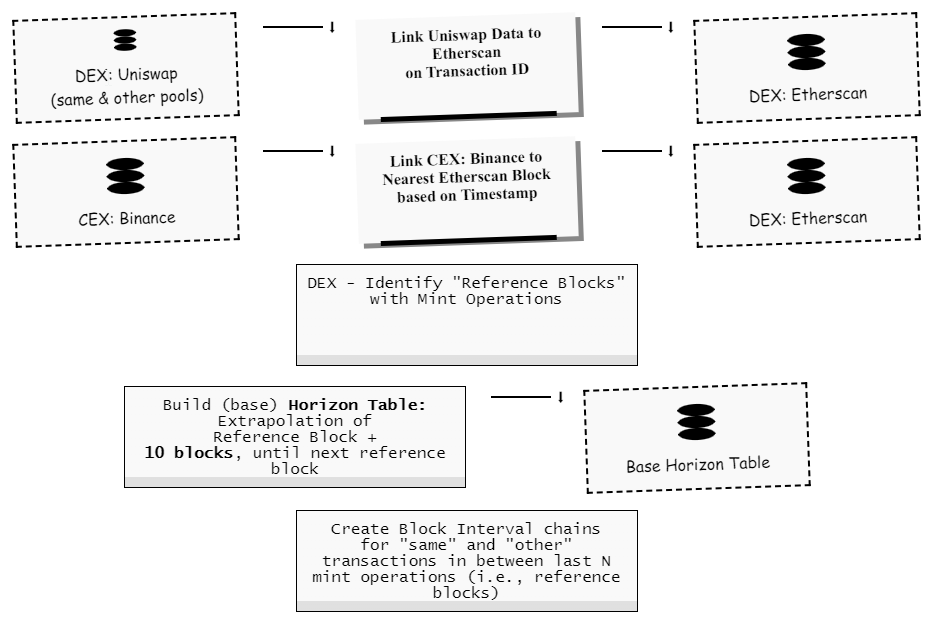
\includegraphics[width=\linewidth]{C:/Users/MatiasVizcaino/repos/6203-DataAnalyticsBusiness-Project/Other Resources/data-diagram/engineer.png}
  \caption{Data Engineering}
  \label{fig:data-diagram-engineer}
  \end{minipage}
  \begin{minipage}{0.45\textwidth}
  \centering
  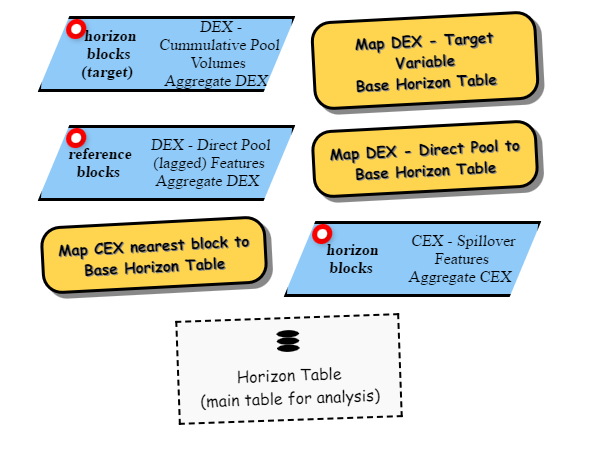
\includegraphics[width=\linewidth]{C:/Users/MatiasVizcaino/repos/6203-DataAnalyticsBusiness-Project/Other Resources/data-diagram/features.png}
  \caption{Feature Engineering}
  \label{fig:data-diagram-features}
  \end{minipage}
\end{figure}

  
  
\begin{table}[htbp]
\centering
\begin{tabular}{|c|c|}
\hline
\textbf{Component} & \textbf{Granularity Level} \\
\hline
DEX target variable & Horizon block level \\
\hline
DEX direct pool features & Reference block level \\
\hline
CEX spillover features & Horizon block level \\
\hline
\end{tabular}
\caption{Granularity Level of Components in Horizon Block Table}
\label{tab:granularity}
\end{table}


\section{Data Profiling Report}

\subsection{Time and Pool Selection}

Our dataset ranges from 01-April-2022 to 30-September-2022. This range includes the Terra-Luna collapse on 20-July-2022, which is a significant event in the DeFi ecosystem, and finished just before The Merge on 04-October-2022, which is a significant event in the Ethereum ecosystem. Refer to Appendix Figure \ref{fig:pool-transactions} for a visualization of the transaction types against time.

We defined a set of pools from the WBTC-WETH exchange, \(P\), where \(p \in P=\{500,3000,\text{both}\}\), facilitating individual, interaction, and aggregate metrics within and across these pools. Transaction types primarily consist of 'burns', 'mints', and 'swaps', with 'swaps' dominating in frequency. The volume of each transaction type varies over time, indicating market dynamics. 

A reference pool \(P_r\) is introduced, with \(P_r \in P\) and \(P_r \neq \text{both}\), denoting a pool where a reference mint operation occurs. This results in \(len(P) * len(P_r)\) possible combinations (i.e., in our case 3*2=6).

The merging process of Uniswap transactions and Etherscan data showed a high match rate of transactions for the six-month analysis period, validating our dataset's integrity. Additional cleaning and integrity checks were carried out on each data source to aid future processing.

\subsection{Reference Blocks and Response variables}

Reference blocks (i.e., those that contain a mint operation) play a crucial role in our analysis. Our dataset houses varying amounts of reference blocks for the 500 (3,242 transactions) and 3000 (4,986 transactions) pools. A particular spike in mint activity in July 2022 raises the need for a deeper probe into potential market events during that period.

\subsection{Block Interval Chains and Block Horizon Table}

We select T=3 to build Block Interval Chains that range from 0 to 3 for the "same" and "other" reference pools \(P_r\), denoted \(C_s\) and \(C_o\) respectively. This will be used to define the (lagged) explanatory variables. Notably, an increasing trend in block time and transaction count from recent to previous intervals was observed.

We select M=10 to build a Horizon Table for each reference mint (refbase, ref500, ref3000), culminating in a total of 118,785 horizons. To boost the robustness of our modeling process, we limit the horizons to a maximum of 30, focusing on the most immediate blocks. Note that which with M=10 it corresponds to about 300 blocks with a total of $\sim$2.3 minutes (given a mean block time of 14 seconds).

\subsection{Response variables}

The response variable in our model, \(Y_{p_{\text{horizon}}}\), denotes the cumulative volume for a pool at a given horizon. Thus, dataset's target variables include 'cum\_volume\_500', 'cum\_volume\_3000', and 'cum\_volume\_base' for each respective reference pool. These variables capture the cumulative volumes across different pools, serving as the backbone for our subsequent modeling.

As described in Section \ref{sec:model-optimization}, we opt to perform a logarithmic transformation using base 10 on the response variables, similar to the approach outlined in \cite{Miori2023}. 
Thus, our response viariable is defined as \(log(Y_{p_{\text{horizon}}}\)).


\subsection{Data Cleaning and Preparation}

We managed missing values in the volatility and avg-USD/rate-USD metrics by replacing null values with zeroes as these would largely relate to the first time interval. Furthermore, we removed highly correlated columns such as such as 'blsame\_2', 'blsame\_3', 'blother\_2', 'blother\_3', 'vol\_0\_1', 'vol\_0\_2' to avoid multicollinearity and aggregated some columns with shared prefixes: 'rate-count-isame\_', 'rate-count-iother\_', 'binance-btc-'. We subsequently dropped the original columns.

During the cleaning process, we tracked data loss, resulting in a negligible reduction of 0.09\% in the observations, indicating successful data cleaning and preservation.

\section{\textbf{In-Depth: Modelling Approach}}

We are studying the correlation between the size of liquidity pools and trading volume using Ordinary Least Squares (OLS) regression models. The OLS method is favored due to its simplicity, interpretability, and widespread use in econometric analysis. Despite the popularity of other models like Poisson regression, negative binomial regression, and logistic regression being available, they are more fitting for count data or binary outcomes, not our continuous outcome of interest. Plus, OLS aligns our research with other academic works\cite{Miori2023}, essential for the scarcity of research in this area. The application of OLS to time-series models involves addressing temporal elements like time trends and seasonal patterns. However, OLS can still be used if our time-series data is believed to follow a linear trend, while considering issues such as autocorrelation and non-stationarity.

\subsection{\textbf{Model Construction and Evaluation}}


The response variable in our model, \(Y_{p_{\text{horizon}}}\), denotes the cumulative volume for a pool at a given horizon. To incorporate temporal dependencies and dynamics in the model, we introduce spot lagged variables of the explanatory variables. These spot lagged variables, denoted as \(\widetilde{i(i-1)}X_s\) and \(\widetilde{i(i-1)}X_o\), represent the values of the explanatory variables at different lags relative to the prediction horizon, for the "same" and "other" pools respectively. We use the Block Interval Chains, denoted \(C_s\) and \(C_o\) respectively, to define these lagged explanatory variables. We standarize the independent variables to make the fitted coefficients easier to compare to each other, because they're all on the same scale. For example, a coefficient of 0.5 means that a one standard deviation increase in the corresponding feature leads to a 0.5 increase in the predicted dependent variable, assuming all other variables are held constant.

The OLS regression model used in our study is expressed as follows:

\begin{equation}
  \log(Y_{p_{\text{horizon}}}) = \beta_0 + \sum_{i=1}^{n} \left(\beta_i^s \cdot \widetilde{i(i-1)}X_s + \beta_i^o \cdot \widetilde{i(i-1)}X_o\right) + \sum_{j=1}^{m} \beta_{n+j} \cdot X_j + \epsilon
  \end{equation}
  
  \begin{table}[h!]
    \centering
    \begin{tabular}{|c|p{0.6\linewidth}|}
    \hline
    \textbf{Variable} & \textbf{Definition} \\
    \hline
    \(\log(Y_{p_{\text{horizon}}})\) & Logarithm of the dependent variable to be predicted at the prediction horizon \(p_{\text{horizon}}\) \\
    \(\beta_0\) & Intercept term: Expected value of \(\log(Y_{p_{\text{horizon}}})\) when all variables are zero \\
    \(\widetilde{i(i-1)}X_s\), \(\widetilde{i(i-1)}X_o\) & Spot lagged variables: Values of \(X\) at different lags relative to the prediction horizon for the "same" and "other" pools, respectively \\
    \(\beta_i^s\), \(\beta_i^o\) & Coefficients associated with each spot lagged variable of \(X\), capturing their effects on the predicted value of \(\log(Y_{p_{\text{horizon}}})\) \\
    \(X_j\) & Additional independent variables or non-lagged variables of \(X\) included in the model \\
    \(\beta_{n+j}\) & Coefficients associated with each additional independent variable, indicating their effects on \(\log(Y_{p_{\text{horizon}}})\) \\
    \(\epsilon\) & Error term or residual: Accounting for unexplained variation in \(\log(Y_{p_{\text{horizon}}})\) not captured by the model \\
    \hline
    \end{tabular}
    \caption{Variable definitions}
    \label{tab:variables}
  \end{table}

We trained and evaluated models for different target variables and horizons, incorporating lagged variables to predict trading volumes at various time horizons. Model performance was assessed using several metrics.

\begin{table}[h!]
  \centering
  \begin{tabular}{|p{0.35\linewidth}|p{0.55\linewidth}|}
  \hline
  \textbf{Metric} & \textbf{Purpose} \\
  \hline
  R-squared & Represents the proportion of the variance for a dependent variable that's explained by an independent variable \\
  Adjusted R-squared & Adjusts the R-squared for the number of predictors in the model \\
  Mean Absolute Error (MAE) & Measures the average magnitude of the errors in a set of predictions \\
  Mean Squared Error (MSE) & Measures the average of the squares of the errors \\
  Root Mean Squared Error (RMSE) & Square root of the MSE, measuring the standard deviation of residuals \\
  \hline
  \end{tabular}
  \caption{Evaluation metrics}
  \label{tab:metrics}
  \end{table}  

\subsection{Train/Test Split and Cross-Validation}

The Train/Test Split methodology assessed the model's ability to generalize to unseen data. Our data set was partitioned into a training set for model training and a test set for evaluating predictive performance.

Cross-validation was applied to assess the OLS model for each horizon. We employed GroupKFold, a form of k-fold cross-validation, to prevent data leakage between training and testing sets. This ensured groups were not split between these sets. We defined groups according to the block reference number. For each fold and up to k=5, the data was split, features standardized, target variables transformed, and an OLS regression model fitted. R-squared and adjusted R-squared were computed for both training and test sets. This process was repeated for each horizon, resulting in trained models and performance metrics. Cross-validation aids in estimating model performance, identifying overfitting, and ensuring reliable generalization across different data subsets.

\subsection{Model Optimization}\label{sec:model-optimization}

Model training involved an iterative "All Horizon Runs" (as in Figure \ref{fig:ols-all-horizons}) approach to explore different modeling techniques, followed by a "Best Horizon Run" to optimize models based on performance. Details on parameters and model configuration can be found on Appendix Table \ref{tab:ols-run-params}. We used the coefficient of determination, R-squared, to gauge model performance, ensuring the model was well-specified and likely to generalize well to new data. The results informed the selection of the most suitable models for predicting the target variables.

\begin{figure}[htbp]
  \centering
  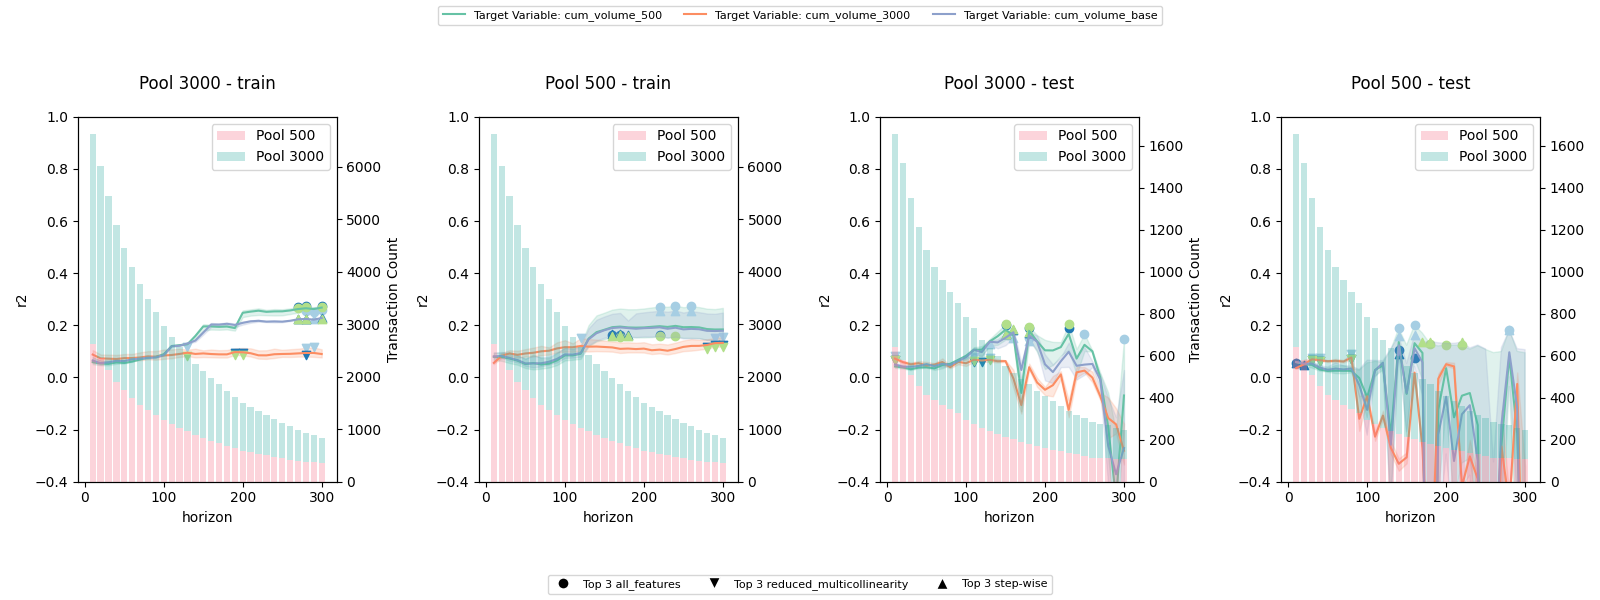
\includegraphics[trim=0 0 0 0, clip, width=\linewidth]{C:/Users/MatiasVizcaino/repos/6203-DataAnalyticsBusiness-Project/Other Resources/OLS_allhorizons_r2.png}
  \caption{OLS Horizon Analysis}
  \label{fig:ols-all-horizons}
\end{figure}

The coefficient of determination, also known as R2 score, quantifies the amount of variance in the dependent variable predictable from the independent variable(s). It ranges from 0 to 1, where 0 means the model explains none of the response data's variability around its mean, and 1 means it explains all the variability. However, R2 can be negative when the model fits poorly and performs worse than a horizontal line (the mean of the dependent variable). This may occur when the model's predictions are consistently far off, causing large errors, or when overfitting occurs on the training data, resulting in poor performance on the test data.

\subsection{Best Horizon Run}\label{sec:model-optimization}
The "Best Horizon Run", focused on identifying the optimal model for specific combinations of horizon and target variables. The 'step-wise' model with parameters \texttt{pool = 3000} and \texttt{target\_variable = 'cum\_volume\_500'} outperformed others in both training and testing environments. We concentrated on \texttt{horizon = 150}, which displayed higher mean $R^2$ values of 0.203 in both training and testing data, indicating superior generalization and predictive accuracy. Other models, in contrast, yielded lower mean $R^2$ values, with some even producing negative values in the testing data, indicating suboptimal performance and poor generalization to unseen data.

The small differences between \(R^2\) and \(R^2_{adj}\) for both the overall data and the specific combination suggest that the 'step-wise' model is not overfitting due to the inclusion of too many predictors. This is a positive indication that the model is well-specified and likely to generalize well to new data. This supports the selection of the 'step-wise' model for the specific combination of parameters, as the model appears to have a good balance between complexity (number of predictors) and performance (as measured by \(R^2_{adj}\)).

In order to manage multicollinearity, we performed a correlation analysis and calculated the Variance Inflation Factor (VIF) as per the equation:

\begin{equation}
  VIF(k) = \frac{1}{1 - R^2_k}
\end{equation}

with $R^2_k$ being the determination coefficient for each predictor.

In Table ~\ref{fig:VIF-analysis}, the condition \( \text{VIF} < b \) compares the Variance Inflation Factor (VIF) to a threshold value \( b \), where values less than 1 indicate low or no multicollinearity, values between 1 and 5 suggest moderate multicollinearity, and values greater than 5 indicate high multicollinearity.

\begin{table}[h]
\centering
\begin{tabular}{lcc}
\hline
 VIF \textless{} b & \textbf{Before Reduction} & \textbf{After Reduction} \\
\hline
\textbf{No/Low} & 0 & 0 \\
\textbf{Moderate} & 21 & 24 \\
\textbf{High} & 22 & 2 \\
\hline
\end{tabular}
\caption{VIF Counts for Thresholds [1, 5, inf]}
\label{fig:VIF-analysis}
\end{table}

Two variables ('rate-count-iother', 'blother\_1') remained with high VIF. Following a correlation analysis, certain highly correlated features were removed. Further reduction of multicollinearity was achieved by aggregating certain intervals, a methodology based on \cite{Miori2023}. See Figure~\ref{fig:correlation-matrix} for the correlation matrix.

\begin{figure}[htbp]
  \centering
  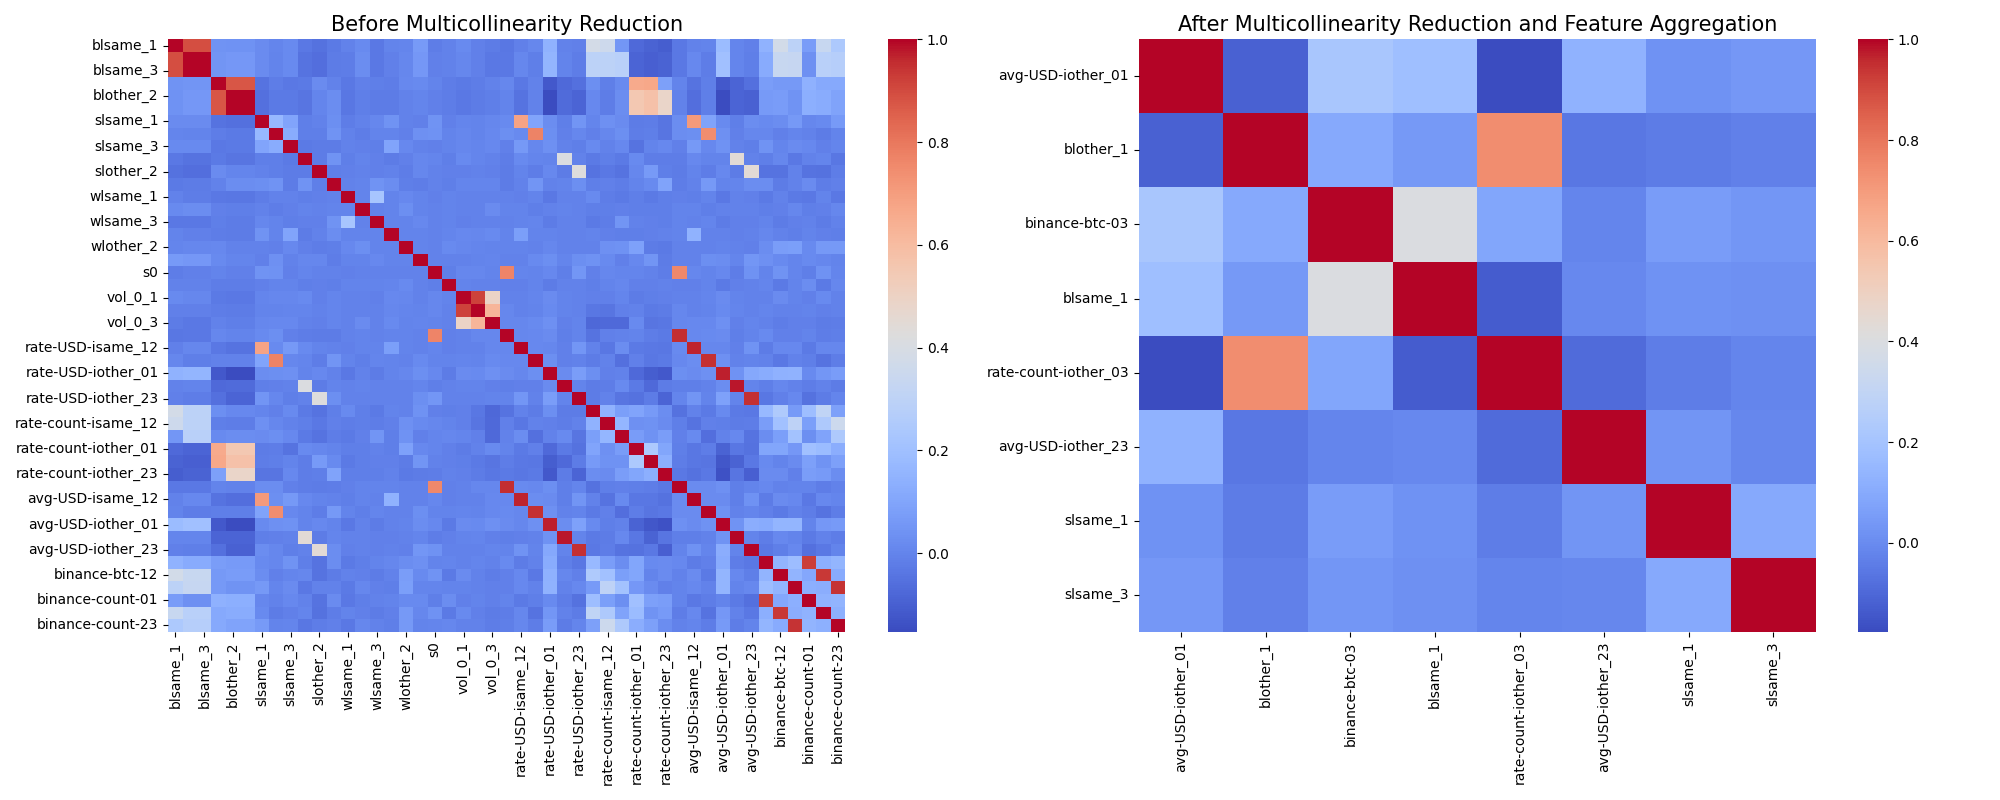
\includegraphics[trim=0 0 0 0, clip, width=0.85\linewidth]{C:/Users/MatiasVizcaino/repos/6203-DataAnalyticsBusiness-Project/Other Resources/correlation_matrix_final.png}
  \caption{Correlation Matrix}
  \label{fig:correlation-matrix}
\end{figure}

\section{\textbf{Feature Selection and Residual Analysis}}

The step-wise feature selection process was used to fit regression models. We systematically removed the least significant features and retrained the model until all remaining features were deemed significant. This approach helps prevent overfitting and enhances model interpretability. Details on number of features in Appendix \ref{tab:number-of-features}.

To identify and address heteroscedasticity, we examine the distribution of error terms. Upon observing a non-linear distribution, we opt to perform a logarithmic transformation using base 10 on the response variables, similar to the approach outlined in \cite{Miori2023}. This transformation aids in stabilizing the variance and aligning the errors with the assumptions of the regression model as illustrated on Figures~\ref{fig:residual-one-horizon} and ~\ref{fig:residual-all-horizons}.

\begin{figure}[htbp]
  \begin{minipage}{0.5\textwidth}
  \centering
  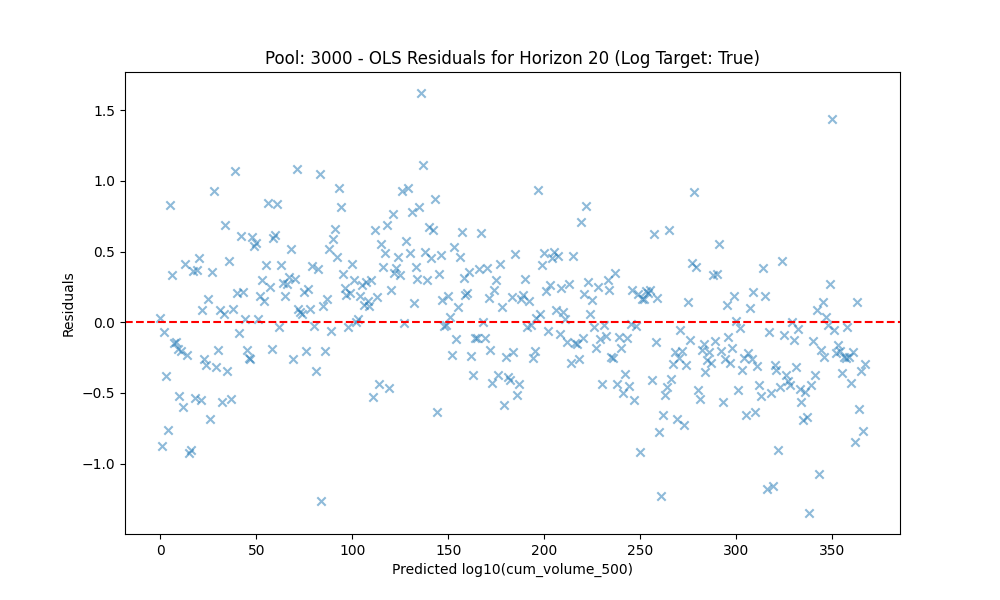
\includegraphics[width=\linewidth]{C:/Users/MatiasVizcaino/repos/6203-DataAnalyticsBusiness-Project/Other Resources/residuals.png}
  \caption{Residuals: One Horizon}
  \label{fig:residual-one-horizon}
  \end{minipage}
  \begin{minipage}{0.45\textwidth}
  \centering
  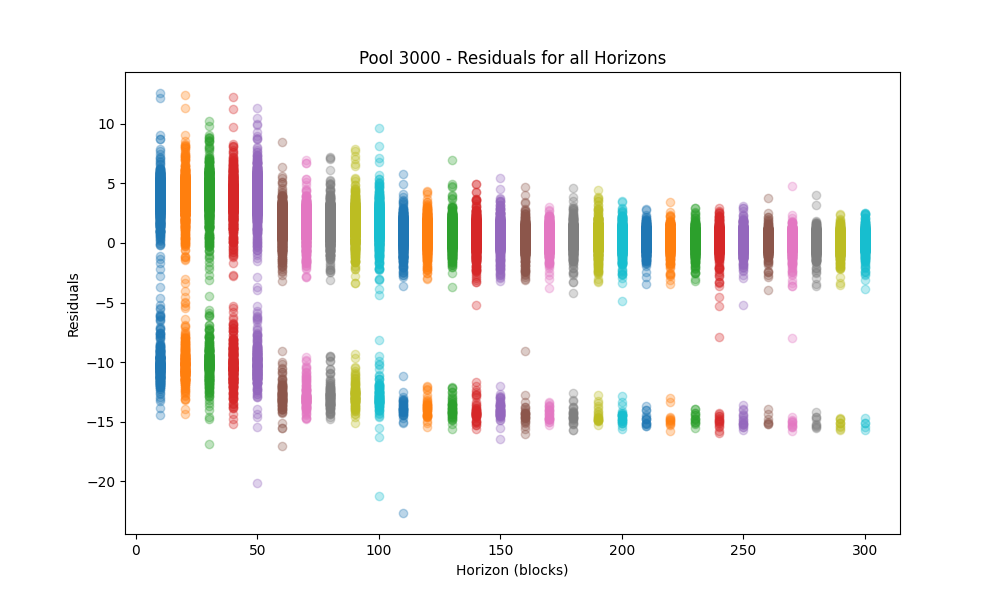
\includegraphics[width=\linewidth]{C:/Users/MatiasVizcaino/repos/6203-DataAnalyticsBusiness-Project/Other Resources/residuals_all_horizons.png}
  \caption{Residuals: All Horizons}
  \label{fig:residual-all-horizons}
  \end{minipage}
  \end{figure}

\subsection{Model Evolution and Detailed Performance Analysis}

Our model's development comprised three distinct stages (see Figure \ref{fig:ols-all-horizons}): an initial stage incorporating all available features, a subsequent phase addressing multicollinearity, and a final stage involving stepwise regression to choose the most statistically significant features.

The model's performance was evaluated based on several criteria: horizon sizes, R-squared values, different data pools, and various target variables. As the horizon extended, predictability, as indicated by \( R^2 \) values, generally decreased, which is consistent with the increased difficulty in predicting further into the future. However, 'all\_features' and 'step-wise' run types with the 'cum\_volume\_500' target variable in the 3000 pool demonstrated consistent high \( R^2 \) values across various horizons, suggesting that our model still exhibited good fit and predictive power even for longer horizons.

Interestingly, we observed negative \( R^2 \) values in some instances, particularly within the test set. This suggests that these models performed worse than a simplistic model based on averages, indicating a potential overfitting issue during the training phase, where the models could not generalize effectively to unseen data.

When comparing the 500 and 3000 pools, the larger pool generally provided higher \( R^2 \) values. This might suggest that reference mints in pool 3000 leads to more accurate predictions. Additionally, for both pools, the 'cum\_volume\_500' target variable typically yielded higher \( R^2 \) values, hinting at a stronger correlation with the selected features.

\subsection{Interpretation of Predictor Coefficients}
For the OLS regression model of "Best Horizon Run" (step-wise model, parameters \texttt{pool = 3000}, \texttt{target\_variable = 'cum\_volume\_500'}), we see a significant overall relationship (F-statistic = 57.38, p \textless{} 0.001). The R-squared value of 0.238 suggests that the predictors account for 23.8\% of the variance in log of 'cum\_volume\_500'.

Post standardization of features, the coefficients for each predictor (Table ~\ref{tab:predictor-coefficients}) express the change in log of 'cum\_volume\_500' linked to a one standard deviation increase in the respective predictor, while other predictors remain constant.

\begin{table}[htbp]
  \centering
  \begin{tabular}{|l|c|c|c|c|}
  \hline
  \textbf{Predictor}        & \textbf{Coef} & \textbf{Std Err} & \textbf{P-value} & \textbf{Significance} \\
  \hline
  Constant                  & 6.1377        & 0.026            & 0.000            & True                  \\
  avg-USD-iother\_01       & 0.1750        & 0.013            & 0.000            & True                  \\
  blother\_1               & -0.1919       & 0.018            & 0.000            & True                  \\
  binance-btc-03          & 0.0976        & 0.013            & 0.000            & True                  \\
  blsame\_1                & -0.0612       & 0.014            & 0.000            & True                  \\
  rate-count-iother\_03    & 0.1115        & 0.019            & 0.000            & True                  \\
  avg-USD-iother\_23       & 0.0294        & 0.012            & 0.016            & True                  \\
  slsame\_1                & 0.0181        & 0.012            & 0.135            & False                 \\
  slsame\_3                & 0.0201        & 0.012            & 0.096            & False                 \\
  \hline
  \end{tabular}
  \caption{Predictor Coefficients}
  \label{tab:predictor-coefficients}
\end{table}

The regression model analysis uses a trigger event - a mint operation in the 'same' pool (3000) - to analyze the impact on the log of cumulative volume ('cum\_volume\_500') of the 'other' pool (500). Post this event, we interpret the effects of the significant predictors:

1. \textbf{Inter-Pool Influence ('avg-USD-iother\_01')}: Higher immediate trading volume in the 'other' pool ('avg-USD-iother\_01') leads to increased cumulative volume in the 'other' pool. 

2. \textbf{Minting Frequency Impact ('blother\_1')}: Decreased frequency of mint operations in the 'other' pool ('blother\_1') corresponds to decreased cumulative volume in the 'other' pool.

3. \textbf{CEX to DEX Spillover ('binance-btc-03')}: Increased BTC trading volume on Binance for up to the third interval post the trigger event ('binance-btc-03') correlates with increased cumulative volume in the 'other' pool. This relationship demonstrates the significant influence of centralized exchange activities on decentralized exchange volumes.

4. \textbf{Same Pool Influence ('blsame\_1')}: Lower frequency of mint operations in the 'same' pool ('blsame\_1') is linked to decreased cumulative volume in the 'other' pool.

5. \textbf{Same Pool Size Impact ('slsame\_1' and 'slsame\_3')}: Although not statistically significant, the size of the previous mint operations in the 'same' pool ('slsame\_1' and 'slsame\_3') potentially impacts the cumulative volume in the 'other' pool.

\section{\textbf{Discussion and Conclusion}}

Our model's time analysis indicates a profound impact of recent events on future outcomes and iteraction within and across pools and exchanges. The immediate past period (t=1 spot and 01 interval) significantly influences future trading volume. It is noteworthy that this finding aligns with established financial theories such as Momentum investing, that suggest recent market behavior often influences subsequent market activity. Consequently, understanding and monitoring the immediate past trading activity could be a vital strategy for predicting and reacting to changes in future trading volumes.

Addressing the study's objectives:

1. Our analysis establishes a relationship between liquidity pool size and trading volume in BTC-ETH liquidity pools. It confirms a direct correlation between pool size and trading volume, highlighting the potential impact of trading activity in one pool on the cumulative volume in another.

2. The influence of liquidity pool size on slippage, particularly considering CEX spillover effects is observed. The BTC trading volume on Binance affects the cumulative volume in the 'other' pool, showing the interplay between CEX and DEX.

3. While this study didn't directly measure the impact of BTC-ETH price volatility on trading volume relative to liquidity pool size, it did indicate how changes in pool size and trading volume are influenced by variables like frequency of mint operations and trading volume on CEX, which could be linked to price volatility.

4. This study identified specific periods/events (e.g., frequency of mint operations in the pool) that significantly \textbf{affect the relationship between BTC-ETH liquidity pool size and trading volume}.

The model demonstrates robustness and good predictive power across different time horizons. Although a slight trend in the residual analysis hints at potential underprediction and overprediction, these findings importantly reinforce the potential of pool sizes as robust predictors of trading volumes. This offers valuable insights for liquidity providers, traders, DeFi platforms, and future research.

\section{Advancements and Implications for Future Research}

This investigation, particularly its contributions to data engineering and feature generation, has significantly propelled the emergent field of financial technology. We would like to acknowledge and extend gratitude towards the authors of "DeFi: modeling and forecasting trading volume on Uniswap v3 liquidity pools (2023)" \cite{Makarov2022,Miori2023} for their invaluable methodology, which guided our replication and validation efforts.

Areas for further investigation include rigorous scrutiny of variables with notable VIF values, a move that could potentially reveal new correlations and optimize the model through feature engineering and redundancy elimination. We also propose exploring non-linear models in light of recent studies hinting at non-linear dependencies \cite{Makarov2022,Miori2023}.

While the OLS regression served as an effective initial model, alternative models accommodating non-linear relationships or time-dependence could bring significant improvements.

We encourage further investigations into price divergences in BTC-ETH exchanges and pools, understanding impermanent loss, and analyzing yield farming protocols. Additionally, adaptations of formulas from \cite{Elsts2021} could deepen the understanding of Uniswap's dynamics.

Finally, addressing challenges and risks associated with DeFi protocols, including economic risks inherent in yield farming and various security risks, is crucial \cite{Xu2023}. This study provides a solid foundation for future research endeavors. We encourage researchers to build upon this work to further the understanding and technological advancement of the DeFi ecosystem.

In our view, future research directions should focus on:

\begin{itemize}
\item \textbf{Model Optimization}: Uncover optimal feature, horizon, and target variable combinations.
\item \textbf{Experimental Adjustments}: Variations in lag/horizon lengths, quadratic features, and structural shifts.
\item \textbf{Temporal Scope}: Study recent time frames and significant industry events.
\end{itemize}


\newpage
\section{Appendix}

Figure \ref{fig:pool-transactions} illustrates the activity history for pools of interest under the scoped period:

\begin{figure}[htbp]
  \centering
  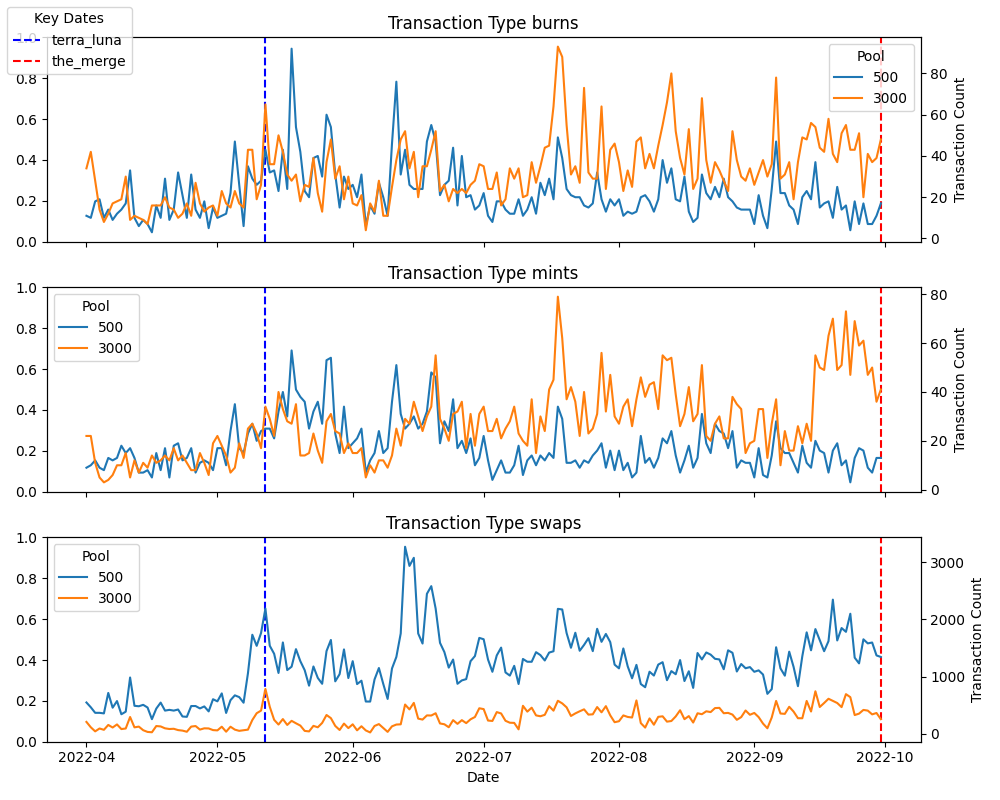
\includegraphics[trim=0 0 0 0, clip, width=\linewidth]{C:/Users/MatiasVizcaino/repos/6203-DataAnalyticsBusiness-Project/Other Resources/transaction_counts.png}
  \caption{Pool Transaction History}
  \label{fig:pool-transactions}
\end{figure}

Table \ref{tab:chains} serves as our block reference table. This is constructed from the transaction data, as we created 8,228 reference blocks that correspond to each mint operation. These blocks were then used to engineer features to calculate metrics for the same pool and other pools. These features capture data about liquidity pools and calculate metrics such as volatility, traded volume rate, trades count, and average volume. To expand the analysis, we have also included lagged features for the previous three mint operations.

\begin{table}[htbp]
  \centering
  \small
  \begin{tabularx}{\linewidth}{|X|r|l|l|}
    \hline
    \textbf{pool} & \textbf{reference block} & \textbf{same\_blockNumberChain} & \textbf{other\_blockNumberChain} \\
    \hline
    500 & 14498564 & [14498564, nan, nan, nan] & [14498564, nan, nan, nan] \\
    500 & 14498699 & [14498699, 14498564, nan, nan] & [14498699, nan, nan, nan] \\
    500 & 14499597 & [14499597, 14498699, 14498564, nan] & [14499597, 14499560, 14499457, 14499198] \\
    500 & 14499836 & [14499836, 14499597, 14498699, 14498564] & [14499836, 14499560, 14499457, 14499198] \\
    500 & 14500355 & [14500355, 14499836, 14499597, 14498699] & [14500355, 14500043, 14499560, 14499457] \\
    ... & ... & ... & ... \\
    3000 & 15648981 & [15648981, 15648330, 15648305, 15648187] & [15648981, 15648887, 15648536, 15646933] \\
    3000 & 15649246 & [15649246, 15648981, 15648330, 15648305] & [15649246, 15649243, 15648887, 15648536] \\
    \hline
  \end{tabularx}
  \caption{Block Interval Chains}
  \label{tab:chains}
\end{table}

We construct a base Horizon Table \ref{tab:horizon-table} with a starting \texttt{horizon\_blockNumber} of each horizon and map it to the closest \texttt{reference\_blockNumber}, defined by mint operations in the block. This base table is joined with the mint aggregated transaction data to generate our target variables and independent variables that are lagged.

\begin{table}[htbp]
  \centering
  \small
  \begin{tabular}{ccccccc}
    \hline
    \textbf{blockNumber} & \textbf{min\_flag} & \textbf{reference\_blockNumber} & \textbf{horizon\_label} & \textbf{cum\_volume\_500} & \textbf{cum\_volume\_3000} \\
    \hline
    108757 & 0 & 15552674 & 9 & 423,485.34 & ...\\
    108758 & 0 & 15552674 & 10 & 423,485.34 & ... \\
    108759 & 1 & 15552772 & 1 & 328,338.73 & ... \\
    108760 & 0 & 15552772 & 2 & 406,084.78 & ... \\
    108761 & 0 & 15552772 & 3 & 536,640.71 & ... \\
    ... & ... & ... & ... & ... & ... \\
    109047 & 0 & 15555464 & 12 & 122,730.73 & ... \\
    109048 & 0 & 15555464 & 13 & 123,650.59 & ... \\
    \hline
  \end{tabular}
  \caption{Example: Horizon Table (reference mint on pool=3000)}
  \label{tab:horizon-table}
\end{table}


Table \ref{tab:number-of-features} provides a summary of the number of features used in different feature selection methods for the analysis, based on the "Best Horizon Run". The three run types included in the table are 'All Features,' 'Multicollinearity Reduction,' and 'Step-Wise Features.' The number of features represents the final set of predictors considered for each run type, indicating the level of feature reduction and selection employed in the modeling process. This table offers insights into the varying complexity and dimensionality of the models implemented in the study.

\begin{table}[htbp]
  \centering
  \small
  \begin{tabular}{|l|r|}
    \hline
    \textbf{Run Type} & \textbf{Number of Features} \\
    \hline
    All Features & 42 \\
    Multicollinearity Reduction & 26 \\
    Step-Wise Features & 8 \\
    \hline
  \end{tabular}
  \caption{Best Horizon: Number of Features by Run Type}
  \label{tab:number-of-features}
\end{table}

To assist in replicability and consistent, we define the "All Horizon Run" and "Best Horizon Run" parameters in Table \ref{tab:ols-run-params}:

\begin{table}[htbp]
  \centering
  \begin{tabularx}{\textwidth}{XccccX}
  \toprule
  \textbf{Run} & \textbf{Pools} & \textbf{Target Variables} & \textbf{M} & \textbf{T} & \textbf{K (CV)} \\
  \midrule
  \textbf{Best Horizon Run} & \multirow{2}{*}{3000} & cum\_volume\_500 & 10 & 3 & 5\\
  \cmidrule(lr){1-1} \cmidrule(lr){3-6}
  \textbf{All Horizon Runs} & 
  \multirow{2}{*}{
  \begin{tabular}{@{}c@{}}
    3000, 500
  \end{tabular}
  } & 
  \begin{tabular}{@{}c@{}}
    cum\_volume\_500, \\
    cum\_volume\_3000, \\
    cum\_volume\_both
  \end{tabular}
  & 10 & 3 & 5\\
  \bottomrule
  \end{tabularx}
  \caption{Run Parameters}
  \label{tab:ols-run-params}
\end{table}


\bibliographystyle{plain} % You could use plain, unsrt, alpha, abbrv etc. 
\bibliography{export}

\end{document}